\documentclass[border=0.25in]{standalone}
\usepackage{tikz}
\usepackage{xcolor}
\usetikzlibrary{shapes.misc, patterns}

\begin{document}
%%%%%%%%%%%%%%%%%%%%%%%%%%%%%%%%%%%%%%%%%%%%%%%%%%
%%%%%%%%%%%%%%%%%%%%%%%%%%%%%%%%%%%%%%%%%%%%%%%%%%
\begin{tabular}{c c}

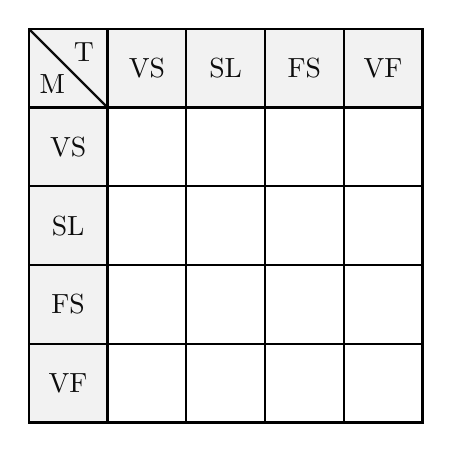
\begin{tikzpicture}
  % Target/Masker
  \node at (0.7, 4.7) {T};
  \node at (0.3, 4.3) {M};
  \draw[thick] (0, 5) -- (1, 4);
  
  % Row labels
  \node at (1.5, 4.5) {VS};
  \node at (2.5, 4.5) {SL};
  \node at (3.5, 4.5) {FS};
  \node at (4.5, 4.5) {VF};
  % Column labels
  \node at (0.5, 3.5) {VS};
  \node at (0.5, 2.5) {SL};
  \node at (0.5, 1.5) {FS};
  \node at (0.5, 0.5) {VF};
  
  % Row 1 (top)
  \draw[thick, draw=black, fill=gray, fill opacity=0.1]
     (0, 4) -- (0, 5) -- (1, 5) -- (1, 4) -- cycle;
  \draw[thick, draw=black, fill=gray, fill opacity=0.1]
     (1, 4) -- (1, 5) -- (2, 5) -- (2, 4) -- cycle;
  \draw[thick, draw=black, fill=gray, fill opacity=0.1]
     (2, 4) -- (2, 5) -- (3, 5) -- (3, 4) -- cycle;
  \draw[thick, draw=black, fill=gray, fill opacity=0.1]
     (3, 4) -- (3, 5) -- (4, 5) -- (4, 4) -- cycle;
  \draw[thick, draw=black, fill=gray, fill opacity=0.1]
     (4, 4) -- (4, 5) -- (5, 5) -- (5, 4) -- cycle;
  % Row 2
  \draw[thick, draw=black, fill=gray, fill opacity=0.1]
     (0, 3) -- (0, 4) -- (1, 4) -- (1, 3) -- cycle;
  \draw[thick, draw=black]
     (1, 3) -- (1, 4) -- (2, 4) -- (2, 3) -- cycle;
  \draw[thick, draw=black]
     (2, 3) -- (2, 4) -- (3, 4) -- (3, 3) -- cycle;
  \draw[thick, draw=black]
     (3, 3) -- (3, 4) -- (4, 4) -- (4, 3) -- cycle;
  \draw[thick, draw=black]
     (4, 3) -- (4, 4) -- (5, 4) -- (5, 3) -- cycle;
  % Row 3
  \draw[thick, draw=black, fill=gray, fill opacity=0.1]
     (0, 2) -- (0, 3) -- (1, 3) -- (1, 2) -- cycle;
  \draw[thick, draw=black]
     (1, 2) -- (1, 3) -- (2, 3) -- (2, 2) -- cycle;
  \draw[thick, draw=black]
     (2, 2) -- (2, 3) -- (3, 3) -- (3, 2) -- cycle;
  \draw[thick, draw=black]
     (3, 2) -- (3, 3) -- (4, 3) -- (4, 2) -- cycle;
  \draw[thick, draw=black]
     (4, 2) -- (4, 3) -- (5, 3) -- (5, 2) -- cycle;
  % Row 4
  \draw[thick, draw=black, fill=gray, fill opacity=0.1]
     (0, 1) -- (0, 2) -- (1, 2) -- (1, 1) -- cycle;
  \draw[thick, draw=black]
     (1, 1) -- (1, 2) -- (2, 2) -- (2, 1) -- cycle;
  \draw[thick, draw=black]
     (2, 1) -- (2, 2) -- (3, 2) -- (3, 1) -- cycle;
  \draw[thick, draw=black]
     (3, 1) -- (3, 2) -- (4, 2) -- (4, 1) -- cycle;
  \draw[thick, draw=black]
     (4, 1) -- (4, 2) -- (5, 2) -- (5, 1) -- cycle;
  % Row 5 (bottom)
  \draw[thick, draw=black, fill=gray, fill opacity=0.1]
     (0, 0) -- (0, 1) -- (1, 1) -- (1, 0) -- cycle;
  \draw[thick, draw=black]
     (1, 0) -- (1, 1) -- (2, 1) -- (2, 0) -- cycle;
  \draw[thick, draw=black]
     (2, 0) -- (2, 1) -- (3, 1) -- (3, 0) -- cycle;
  \draw[thick, draw=black]
     (3, 0) -- (3, 1) -- (4, 1) -- (4, 0) -- cycle;
  \draw[thick, draw=black]
     (4, 0) -- (4, 1) -- (5, 1) -- (5, 0) -- cycle;
\end{tikzpicture}
&



%%% Pattern fill
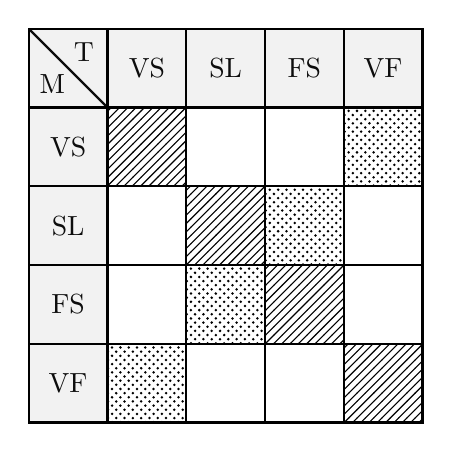
\begin{tikzpicture}
  % Target/Masker
  \node at (0.7, 4.7) {T};
  \node at (0.3, 4.3) {M};
  \draw[thick] (0, 5) -- (1, 4);
  
  % Row labels
  \node at (1.5, 4.5) {VS};
  \node at (2.5, 4.5) {SL};
  \node at (3.5, 4.5) {FS};
  \node at (4.5, 4.5) {VF};
  % Column labels
  \node at (0.5, 3.5) {VS};
  \node at (0.5, 2.5) {SL};
  \node at (0.5, 1.5) {FS};
  \node at (0.5, 0.5) {VF};
  
  % Row 1 (top)
  \draw[thick, draw=black, fill=gray, fill opacity=0.1]
     (0, 4) -- (0, 5) -- (1, 5) -- (1, 4) -- cycle;
  \draw[thick, draw=black, fill=gray, fill opacity=0.1]
     (1, 4) -- (1, 5) -- (2, 5) -- (2, 4) -- cycle;
  \draw[thick, draw=black, fill=gray, fill opacity=0.1]
     (2, 4) -- (2, 5) -- (3, 5) -- (3, 4) -- cycle;
  \draw[thick, draw=black, fill=gray, fill opacity=0.1]
     (3, 4) -- (3, 5) -- (4, 5) -- (4, 4) -- cycle;
  \draw[thick, draw=black, fill=gray, fill opacity=0.1]
     (4, 4) -- (4, 5) -- (5, 5) -- (5, 4) -- cycle;
  % Row 2
  \draw[thick, draw=black, fill=gray, fill opacity=0.1]
     (0, 3) -- (0, 4) -- (1, 4) -- (1, 3) -- cycle;
  \draw[thick, draw=black, pattern=north east lines]
     (1, 3) -- (1, 4) -- (2, 4) -- (2, 3) -- cycle;
  \draw[thick, draw=black]
     (2, 3) -- (2, 4) -- (3, 4) -- (3, 3) -- cycle;
  \draw[thick, draw=black]
     (3, 3) -- (3, 4) -- (4, 4) -- (4, 3) -- cycle;
  \draw[thick, draw=black, pattern=crosshatch dots]
     (4, 3) -- (4, 4) -- (5, 4) -- (5, 3) -- cycle;
  % Row 3
  \draw[thick, draw=black, fill=gray, fill opacity=0.1]
     (0, 2) -- (0, 3) -- (1, 3) -- (1, 2) -- cycle;
  \draw[thick, draw=black]
     (1, 2) -- (1, 3) -- (2, 3) -- (2, 2) -- cycle;
  \draw[thick, draw=black, pattern=north east lines]
     (2, 2) -- (2, 3) -- (3, 3) -- (3, 2) -- cycle;
  \draw[thick, draw=black, pattern=crosshatch dots]
     (3, 2) -- (3, 3) -- (4, 3) -- (4, 2) -- cycle;
  \draw[thick, draw=black]
     (4, 2) -- (4, 3) -- (5, 3) -- (5, 2) -- cycle;
  % Row 4
  \draw[thick, draw=black, fill=gray, fill opacity=0.1]
     (0, 1) -- (0, 2) -- (1, 2) -- (1, 1) -- cycle;
  \draw[thick, draw=black]
     (1, 1) -- (1, 2) -- (2, 2) -- (2, 1) -- cycle;
  \draw[thick, draw=black, pattern=crosshatch dots]
     (2, 1) -- (2, 2) -- (3, 2) -- (3, 1) -- cycle;
  \draw[thick, draw=black, pattern=north east lines]
     (3, 1) -- (3, 2) -- (4, 2) -- (4, 1) -- cycle;
  \draw[thick, draw=black]
     (4, 1) -- (4, 2) -- (5, 2) -- (5, 1) -- cycle;
  % Row 5 (bottom)
  \draw[thick, draw=black, fill=gray, fill opacity=0.1]
     (0, 0) -- (0, 1) -- (1, 1) -- (1, 0) -- cycle;
  \draw[thick, draw=black, pattern=crosshatch dots]
     (1, 0) -- (1, 1) -- (2, 1) -- (2, 0) -- cycle;
  \draw[thick, draw=black]
     (2, 0) -- (2, 1) -- (3, 1) -- (3, 0) -- cycle;
  \draw[thick, draw=black]
     (3, 0) -- (3, 1) -- (4, 1) -- (4, 0) -- cycle;
  \draw[thick, draw=black, pattern=north east lines]
     (4, 0) -- (4, 1) -- (5, 1) -- (5, 0) -- cycle;
\end{tikzpicture}

\vspace{0.25in}
\\



%%% Color fill
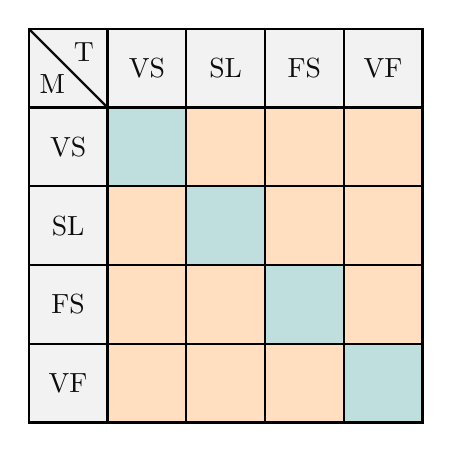
\begin{tikzpicture}
  % Target/Masker
  \node at (0.7, 4.7) {T};
  \node at (0.3, 4.3) {M};
  \draw[thick] (0, 5) -- (1, 4);
  
  % Row labels
  \node at (1.5, 4.5) {VS};
  \node at (2.5, 4.5) {SL};
  \node at (3.5, 4.5) {FS};
  \node at (4.5, 4.5) {VF};
  % Column labels
  \node at (0.5, 3.5) {VS};
  \node at (0.5, 2.5) {SL};
  \node at (0.5, 1.5) {FS};
  \node at (0.5, 0.5) {VF};
  
  % Row 1 (top)
  \draw[thick, draw=black, fill=gray, fill opacity=0.1]
     (0, 4) -- (0, 5) -- (1, 5) -- (1, 4) -- cycle;
  \draw[thick, draw=black, fill=gray, fill opacity=0.1]
     (1, 4) -- (1, 5) -- (2, 5) -- (2, 4) -- cycle;
  \draw[thick, draw=black, fill=gray, fill opacity=0.1]
     (2, 4) -- (2, 5) -- (3, 5) -- (3, 4) -- cycle;
  \draw[thick, draw=black, fill=gray, fill opacity=0.1]
     (3, 4) -- (3, 5) -- (4, 5) -- (4, 4) -- cycle;
  \draw[thick, draw=black, fill=gray, fill opacity=0.1]
     (4, 4) -- (4, 5) -- (5, 5) -- (5, 4) -- cycle;
  % Row 2
  \draw[thick, draw=black, fill=gray, fill opacity=0.1]
     (0, 3) -- (0, 4) -- (1, 4) -- (1, 3) -- cycle;
  \draw[thick, draw=black, fill=teal, fill opacity=0.25]
     (1, 3) -- (1, 4) -- (2, 4) -- (2, 3) -- cycle;
  \draw[thick, draw=black, fill=orange, fill opacity=0.25]
     (2, 3) -- (2, 4) -- (3, 4) -- (3, 3) -- cycle;
  \draw[thick, draw=black, fill=orange, fill opacity=0.25]
     (3, 3) -- (3, 4) -- (4, 4) -- (4, 3) -- cycle;
  \draw[thick, draw=black, fill=orange, fill opacity=0.25]
     (4, 3) -- (4, 4) -- (5, 4) -- (5, 3) -- cycle;
  % Row 3
  \draw[thick, draw=black, fill=gray, fill opacity=0.1]
     (0, 2) -- (0, 3) -- (1, 3) -- (1, 2) -- cycle;
  \draw[thick, draw=black, fill=orange, fill opacity=0.25]
     (1, 2) -- (1, 3) -- (2, 3) -- (2, 2) -- cycle;
  \draw[thick, draw=black, fill=teal, fill opacity=0.25]
     (2, 2) -- (2, 3) -- (3, 3) -- (3, 2) -- cycle;
  \draw[thick, draw=black, fill=orange, fill opacity=0.25]
     (3, 2) -- (3, 3) -- (4, 3) -- (4, 2) -- cycle;
  \draw[thick, draw=black, fill=orange, fill opacity=0.25]
     (4, 2) -- (4, 3) -- (5, 3) -- (5, 2) -- cycle;
  % Row 4
  \draw[thick, draw=black, fill=gray, fill opacity=0.1]
     (0, 1) -- (0, 2) -- (1, 2) -- (1, 1) -- cycle;
  \draw[thick, draw=black, fill=orange, fill opacity=0.25]
     (1, 1) -- (1, 2) -- (2, 2) -- (2, 1) -- cycle;
  \draw[thick, draw=black, fill=orange, fill opacity=0.25]
     (2, 1) -- (2, 2) -- (3, 2) -- (3, 1) -- cycle;
  \draw[thick, draw=black, fill=teal, fill opacity=0.25]
     (3, 1) -- (3, 2) -- (4, 2) -- (4, 1) -- cycle;
  \draw[thick, draw=black, fill=orange, fill opacity=0.25]
     (4, 1) -- (4, 2) -- (5, 2) -- (5, 1) -- cycle;
  % Row 5 (bottom)
  \draw[thick, draw=black, fill=gray, fill opacity=0.1]
     (0, 0) -- (0, 1) -- (1, 1) -- (1, 0) -- cycle;
  \draw[thick, draw=black, fill=orange, fill opacity=0.25]
     (1, 0) -- (1, 1) -- (2, 1) -- (2, 0) -- cycle;
  \draw[thick, draw=black, fill=orange, fill opacity=0.25]
     (2, 0) -- (2, 1) -- (3, 1) -- (3, 0) -- cycle;
  \draw[thick, draw=black, fill=orange, fill opacity=0.25]
     (3, 0) -- (3, 1) -- (4, 1) -- (4, 0) -- cycle;
  \draw[thick, draw=black, fill=teal, fill opacity=0.25]
     (4, 0) -- (4, 1) -- (5, 1) -- (5, 0) -- cycle;
\end{tikzpicture}
&



%%% Color and pattern fill
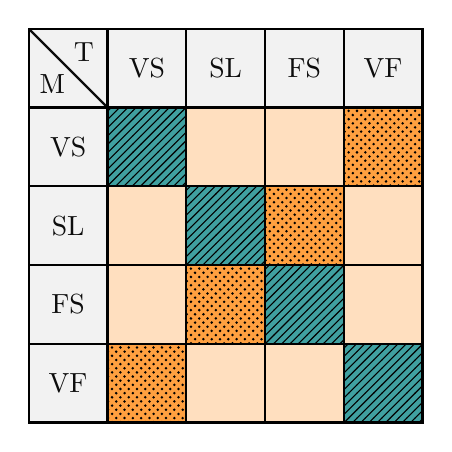
\begin{tikzpicture}
  % Target/Masker
  \node at (0.7, 4.7) {T};
  \node at (0.3, 4.3) {M};
  \draw[thick] (0, 5) -- (1, 4);
  
  % Row labels
  \node at (1.5, 4.5) {VS};
  \node at (2.5, 4.5) {SL};
  \node at (3.5, 4.5) {FS};
  \node at (4.5, 4.5) {VF};
  % Column labels
  \node at (0.5, 3.5) {VS};
  \node at (0.5, 2.5) {SL};
  \node at (0.5, 1.5) {FS};
  \node at (0.5, 0.5) {VF};
  
  % Row 1 (top)
  \draw[thick, draw=black, fill=gray, fill opacity=0.1]
     (0, 4) -- (0, 5) -- (1, 5) -- (1, 4) -- cycle;
  \draw[thick, draw=black, fill=gray, fill opacity=0.1]
     (1, 4) -- (1, 5) -- (2, 5) -- (2, 4) -- cycle;
  \draw[thick, draw=black, fill=gray, fill opacity=0.1]
     (2, 4) -- (2, 5) -- (3, 5) -- (3, 4) -- cycle;
  \draw[thick, draw=black, fill=gray, fill opacity=0.1]
     (3, 4) -- (3, 5) -- (4, 5) -- (4, 4) -- cycle;
  \draw[thick, draw=black, fill=gray, fill opacity=0.1]
     (4, 4) -- (4, 5) -- (5, 5) -- (5, 4) -- cycle;
  % Row 2
  \draw[thick, draw=black, fill=gray, fill opacity=0.1]
     (0, 3) -- (0, 4) -- (1, 4) -- (1, 3) -- cycle;
  \draw[thick, draw=black, fill=teal, fill opacity=0.75]
     (1, 3) -- (1, 4) -- (2, 4) -- (2, 3) -- cycle;
  \draw[thick, draw=black, pattern=north east lines]
     (1, 3) -- (1, 4) -- (2, 4) -- (2, 3) -- cycle;
  \draw[thick, draw=black, fill=orange, fill opacity=0.25]
     (2, 3) -- (2, 4) -- (3, 4) -- (3, 3) -- cycle;
  \draw[thick, draw=black, fill=orange, fill opacity=0.25]
     (3, 3) -- (3, 4) -- (4, 4) -- (4, 3) -- cycle;
  \draw[thick, draw=black, fill=orange, fill opacity=0.75]
     (4, 3) -- (4, 4) -- (5, 4) -- (5, 3) -- cycle;
  \draw[thick, draw=black, pattern=crosshatch dots]
     (4, 3) -- (4, 4) -- (5, 4) -- (5, 3) -- cycle;
  % Row 3
  \draw[thick, draw=black, fill=gray, fill opacity=0.1]
     (0, 2) -- (0, 3) -- (1, 3) -- (1, 2) -- cycle;
  \draw[thick, draw=black, fill=orange, fill opacity=0.25]
     (1, 2) -- (1, 3) -- (2, 3) -- (2, 2) -- cycle;
  \draw[thick, draw=black, fill=teal, fill opacity=0.75]
     (2, 2) -- (2, 3) -- (3, 3) -- (3, 2) -- cycle;
  \draw[thick, draw=black, pattern=north east lines]
     (2, 2) -- (2, 3) -- (3, 3) -- (3, 2) -- cycle;
  \draw[thick, draw=black, fill=orange, fill opacity=0.75]
     (3, 2) -- (3, 3) -- (4, 3) -- (4, 2) -- cycle;
  \draw[thick, draw=black, pattern=crosshatch dots]
     (3, 2) -- (3, 3) -- (4, 3) -- (4, 2) -- cycle;
  \draw[thick, draw=black, fill=orange, fill opacity=0.25]
     (4, 2) -- (4, 3) -- (5, 3) -- (5, 2) -- cycle;
  % Row 4
  \draw[thick, draw=black, fill=gray, fill opacity=0.1]
     (0, 1) -- (0, 2) -- (1, 2) -- (1, 1) -- cycle;
  \draw[thick, draw=black, fill=orange, fill opacity=0.25]
     (1, 1) -- (1, 2) -- (2, 2) -- (2, 1) -- cycle;
  \draw[thick, draw=black, fill=orange, fill opacity=0.75]
     (2, 1) -- (2, 2) -- (3, 2) -- (3, 1) -- cycle;
  \draw[thick, draw=black, pattern=crosshatch dots]
     (2, 1) -- (2, 2) -- (3, 2) -- (3, 1) -- cycle;
  \draw[thick, draw=black, fill=teal, fill opacity=0.75]
     (3, 1) -- (3, 2) -- (4, 2) -- (4, 1) -- cycle;
  \draw[thick, draw=black, pattern=north east lines]
     (3, 1) -- (3, 2) -- (4, 2) -- (4, 1) -- cycle;
  \draw[thick, draw=black, fill=orange, fill opacity=0.25]
     (4, 1) -- (4, 2) -- (5, 2) -- (5, 1) -- cycle;
  % Row 5 (bottom)
  \draw[thick, draw=black, fill=gray, fill opacity=0.1]
     (0, 0) -- (0, 1) -- (1, 1) -- (1, 0) -- cycle;
  \draw[thick, draw=black, fill=orange, fill opacity=0.75]
     (1, 0) -- (1, 1) -- (2, 1) -- (2, 0) -- cycle;
  \draw[thick, draw=black, pattern=crosshatch dots]
     (1, 0) -- (1, 1) -- (2, 1) -- (2, 0) -- cycle;
  \draw[thick, draw=black, fill=orange, fill opacity=0.25]
     (2, 0) -- (2, 1) -- (3, 1) -- (3, 0) -- cycle;
  \draw[thick, draw=black, fill=orange, fill opacity=0.25]
     (3, 0) -- (3, 1) -- (4, 1) -- (4, 0) -- cycle;
  \draw[thick, draw=black, fill=teal, fill opacity=0.75]
     (4, 0) -- (4, 1) -- (5, 1) -- (5, 0) -- cycle;
  \draw[thick, draw=black, pattern=north east lines]
     (4, 0) -- (4, 1) -- (5, 1) -- (5, 0) -- cycle;
\end{tikzpicture}

\end{tabular}

%%%%%%%%%%%%%%%%%%%%%%%%%%%%%%%%%%%%%%%%%%%%%%%%%%
%%%%%%%%%%%%%%%%%%%%%%%%%%%%%%%%%%%%%%%%%%%%%%%%%%
\end{document}